% !TEX program = pdflatex
% AI-Assisted Hacking: Key to Interoperability or Security Nightmare?
% arXiv-friendly: \documentclass{article}, only widely-available packages.
\documentclass[11pt,a4paper]{article}

\usepackage[utf8]{inputenc}
\usepackage[T1]{fontenc}
\usepackage{lmodern}
\usepackage[english]{babel}
\usepackage[margin=1in]{geometry}
\usepackage{microtype}
\usepackage{graphicx}
\usepackage{booktabs}
\usepackage{caption}
\usepackage{subcaption}
\usepackage{xcolor}
\usepackage{csquotes}
\usepackage[numbers,sort&compress]{natbib}
\usepackage{hyperref}
\hypersetup{
  colorlinks=true,
  linkcolor=black,
  citecolor=black,
  urlcolor=black,
  pdftitle={AI-Assisted Hacking: Key to Interoperability or Security Nightmare?},
  pdfauthor={}
}

\graphicspath{{figures/}}

\title{AI-Assisted Hacking: Key to Interoperability or Security Nightmare?}
\author{}
\date{\today}

\begin{document}
\maketitle

\begin{abstract}
This paper investigates how modern large language models collapse the traditional ``effort gap'' in reverse engineering. Through two case studies, we show how AI-assisted analysis turns theoretical protocol knowledge into practical, replicable local integrations, and we assess whether this is a force for interoperability or a systemic security risk.
\end{abstract}

\section{Introduction}
The rise of proprietary IoT ecosystems has made local interoperability difficult by design. This study asks:
\begin{quote}
Is AI-assisted hacking a key to interoperability, or does it turn security through obscurity into a security nightmare?
\end{quote}
This paper argues that the central barrier is not a lack of technical capability but the activation energy required to move from theory to practice. With AI, that barrier is shrinking, and the implications are both liberating and dangerous (Figure~\ref{fig:effort-gap}).

\begin{figure}[t]
  \centering
  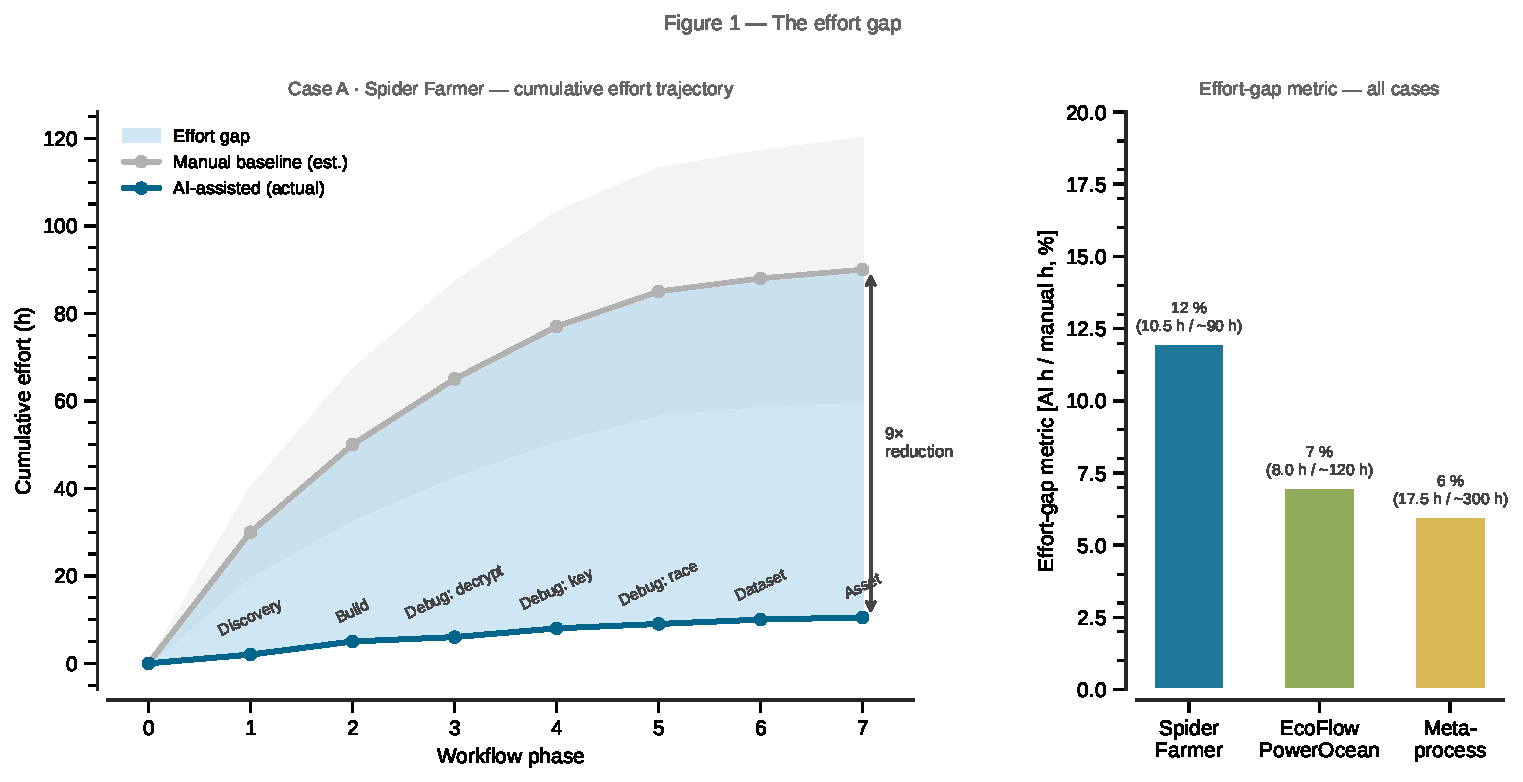
\includegraphics[width=0.92\linewidth]{fig1-effort-gap.pdf}
  \caption{\textbf{The effort gap.} Cumulative human effort to reach a working local integration across phases of a reverse-engineering project. AI-assisted analysis flattens the curve: the activation energy that historically gated practical interoperability work collapses, leaving a wide effort gap between the two trajectories.}
  \label{fig:effort-gap}
\end{figure}

\section{Contributions}
\begin{itemize}
  \item Define the ``effort gap'' in modern IoT reverse engineering.
  \item Present two empirical case studies: Spider Farmer and EcoFlow PowerOcean.
  \item Propose a methodology for auditing AI-assisted research, including artifact analysis, documentation comparison, and commit-history review.
  \item Evaluate interoperability benefits against dual-use security risks.
\end{itemize}

\section{Related Work}
\begin{itemize}
  \item Security-through-obscurity and IoT vendor lock-in.
  \item AI and language models in software reverse engineering.
  \item Right-to-repair, local control, and privacy in smart home systems.
\end{itemize}

The activation-energy framing is central to this paper (Figure~\ref{fig:boredom-barrier}): the thermodynamic endpoint --- a working integration --- is unchanged, but AI-assisted analysis lowers the barrier separating theory from practice.

\begin{figure}[t]
  \centering
  
\includegraphics[width=0.92\linewidth]{fig2-boredom-barrier.pdf}
  \caption{\textbf{The boredom barrier.} Reaction-coordinate view of a reverse-engineering project. The thermodynamic endpoint --- a working integration --- is unchanged. AI-assisted analysis lowers the activation energy $E_\mathrm{a}$ by absorbing the rote, low-novelty work where most projects historically stalled.}
  \label{fig:boredom-barrier}
\end{figure}

\section{Case Study A: Spider Farmer}
\begin{itemize}
  \item System description and vendor control model.
  \item AI-assisted APK and protocol analysis workflow.
  \item Results: local Home Assistant integration and practical interoperability.
\end{itemize}

Figure~\ref{fig:case-spider-farmer} summarises the workflow.

\begin{figure}[t]
  \centering
  
\includegraphics[width=0.92\linewidth]{fig3-spider-farmer.pdf}
  \caption{\textbf{Case study A --- Spider Farmer.} The vendor surface (APK, on-device traffic, undocumented cloud endpoints) is collapsed by an LLM-assisted analysis loop into a working local Home Assistant integration. Prompt logs and transcripts are preserved as auditable research artifacts.}
  \label{fig:case-spider-farmer}
\end{figure}

\section{Case Study B: EcoFlow PowerOcean}
\begin{itemize}
  \item Energy management use case and system complexity.
  \item AI-assisted reverse engineering of undocumented APIs, packet formats, and device telemetry.
  \item Results: local monitoring, control, and reduced reliance on cloud services.
\end{itemize}

Figure~\ref{fig:case-ecoflow} contrasts the vendor default (cloud-bound) with the AI-assisted local-control architecture.

\begin{figure}[t]
  \centering
  
\includegraphics[width=0.92\linewidth]{fig4-ecoflow.pdf}
  \caption{\textbf{Case study B --- EcoFlow PowerOcean.} Left: the vendor default routes home telemetry and user commands through a required cloud hop. Right: AI-assisted reverse engineering yields a protocol map and a local broker on the LAN, making the cloud optional and restoring data ownership.}
  \label{fig:case-ecoflow}
\end{figure}

\section{Methodology}
\begin{itemize}
  \item Data acquisition: APKs, firmware, packet captures, documentation, and prompt logs.
  \item AI-assisted analysis: combining generated and existing documentation with code and protocol inspection, including exported conversation transcripts as research artifacts.
  \item Version history review: commit and branch analysis to understand development evolution and research provenance.
  \item Validation: reproducing findings and documenting failed attempts.
\end{itemize}

The four-stage pipeline is summarised in Figure~\ref{fig:methodology}.

\begin{figure}[t]
  \centering
  
\includegraphics[width=0.92\linewidth]{fig5-methodology.pdf}
  \caption{\textbf{Methodology.} The four-stage pipeline used in both case studies: Acquire (artifacts \& prompt logs) $\rightarrow$ Analyse (LLM-assisted) $\rightarrow$ Audit (provenance, commit history, transcript review) $\rightarrow$ Validate (reproduce, replay, log failures), with an explicit feedback loop from validation back into analysis.}
  \label{fig:methodology}
\end{figure}

\section{Discussion: Interoperability vs.\ Security Nightmare}
\begin{itemize}
  \item The democratization of reverse engineering and the new ``boredom barrier.''
  \item Consumer sovereignty, right-to-repair, and local data ownership.
  \item Dual-use risks: vendor attack surface, rapid protocol discovery, and abuse potential.
  \item The future of IoT security: open APIs, zero-trust, and accountable design.
\end{itemize}

The dual-use character of the technology is shown in Figure~\ref{fig:dual-use}: AI broadens the reachable distribution of outcomes, both legitimate and abusive. The structural answer is a shift in threat model (Figure~\ref{fig:threat-models}), away from a single perimeter protecting implicitly trusted devices and toward authenticated, scoped access at every hop.

\begin{figure}[t]
  \centering
  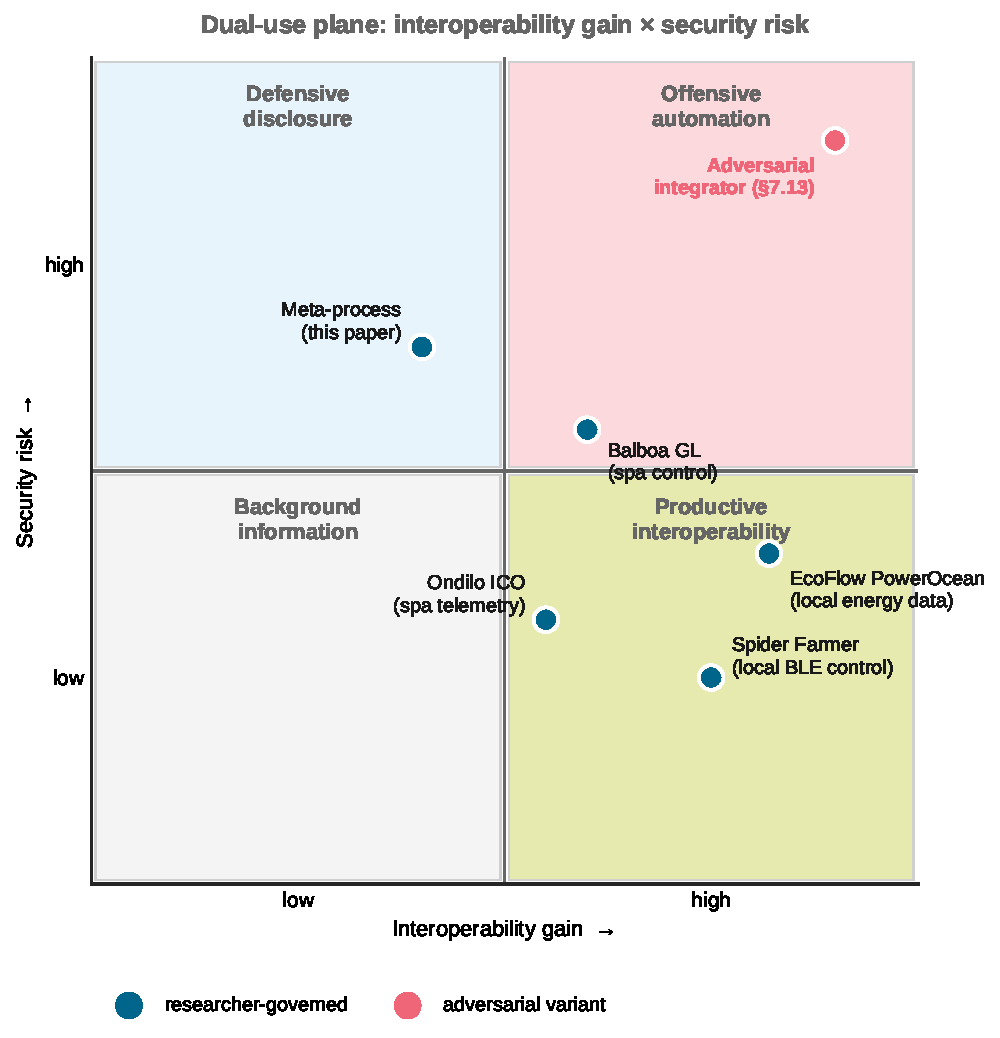
\includegraphics[width=0.92\linewidth]{fig6-dual-use.pdf}
  \caption{\textbf{Dual-use map.} Outcomes of AI-assisted reverse engineering plotted by interoperability gain ($x$) versus security risk ($y$). The dashed envelope shows how AI broadens the reachable distribution: legitimate use cases gain reach, but so do high-risk ones --- the policy question is which quadrants to incentivise.}
  \label{fig:dual-use}
\end{figure}

\begin{figure}[t]
  \centering
  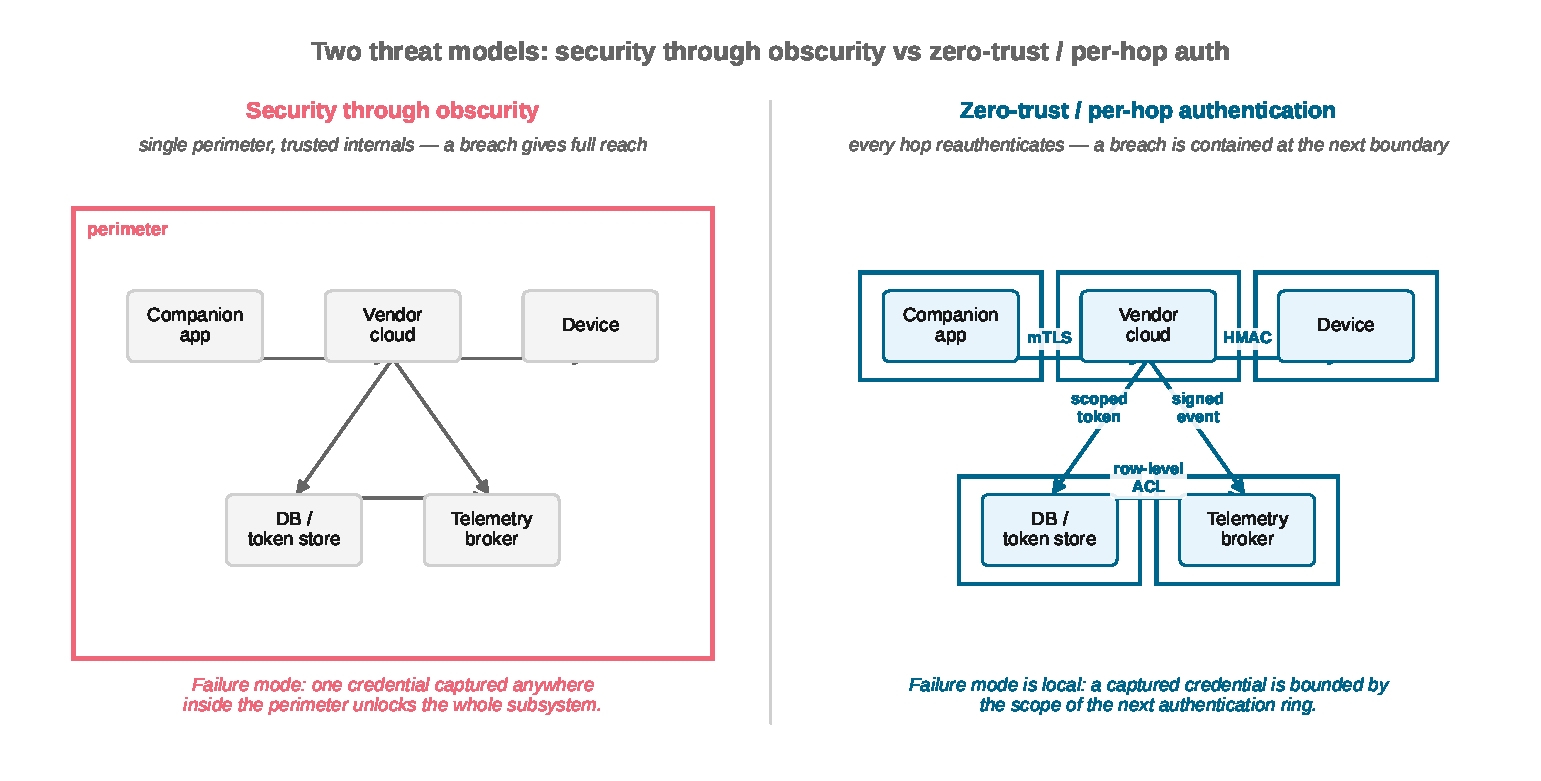
\includegraphics[width=0.92\linewidth]{fig7-threat-models.pdf}
  \caption{\textbf{Two threat models.} Left: a single perimeter protects implicitly trusted devices --- once breached, the whole system is exposed. Right: every hop is authenticated against a published specification; a breach stays local. AI-assisted reverse engineering punctures the left model and rewards systems built on the right.}
  \label{fig:threat-models}
\end{figure}

\section{Conclusion}
AI-assisted hacking is a double-edged force: it enables local interoperability and user freedom while exposing the fragility of security through obscurity. The path forward is not to ban AI, but to design systems that do not depend on secrecy.

\section{Future Work}
\begin{itemize}
  \item Expand empirical evaluation to additional devices and vendors.
  \item Develop reproducible prompt templates and audit workflows.
  \item Propose a responsible disclosure framework for AI-assisted reverse engineering.
\end{itemize}

\bibliographystyle{plainnat}
\bibliography{references}

\end{document}
